% Lab 05 - "Robot poszukujacy" - raport (1 strona A4).
% Kompilacja: pdflatex raport.tex  (Overleaf: domyslny pdfLaTeX)  lub  xelatex raport.tex
% Strona 2 z wykresem bledow jest opcjonalna: \dodatektrue / \dodatekfalse ponizej.
\documentclass[a4paper,10pt]{article}

\newif\ifdodatek
\dodatekfalse            % \dodatektrue = dolacz strone 2 z wykresem bledow (wykres_bledow.pdf)

\usepackage{iftex}
\ifPDFTeX
  \usepackage[T1]{fontenc}
  \usepackage[utf8]{inputenc}
  \usepackage{lmodern}
  \usepackage{tgheros}
\else
  \usepackage{fontspec}
  \setmainfont{texgyreheros}[Extension=.otf, UprightFont=*-regular, BoldFont=*-bold,
    ItalicFont=*-italic, BoldItalicFont=*-bolditalic]
\fi
\renewcommand{\familydefault}{\sfdefault}
\usepackage[polish]{babel}
\usepackage[autostyle]{csquotes}
\usepackage[a4paper,top=8mm,bottom=7mm,left=9mm,right=9mm]{geometry}
\usepackage[table]{xcolor}
\usepackage{multicol}
\usepackage{tabularx}
\usepackage{array}
\usepackage{enumitem}
\usepackage{titlesec}
\usepackage{graphicx}
\usepackage{amsmath}
\usepackage{tikz}
\usetikzlibrary{arrows.meta}
\usepackage{microtype}

\pagestyle{empty}
\definecolor{accent}{HTML}{1F5FA8}
\definecolor{ink}{HTML}{1B1F24}
\definecolor{muted}{HTML}{5B6470}
\definecolor{line}{HTML}{C9D1DA}
\definecolor{bgtwo}{HTML}{F2F5F9}
\definecolor{ownfill}{HTML}{E3EEFB}
\definecolor{boxline}{HTML}{3B4A5A}
\definecolor{extline}{HTML}{7A8794}

% --- typografia: 8.1 pt, jak w wersji HTML
\newcommand{\bodyfont}{\fontsize{8.1}{9.9}\selectfont}
\newcommand{\code}[1]{\texttt{\fontsize{7.2}{9}\selectfont\detokenize{#1}}}
\newcommand{\ra}{\ensuremath{\rightarrow}}
\newcommand{\Tr}[2]{\ensuremath{T^{\mathrm{#1}}_{\mathrm{#2}}}}
\titleformat{\section}{\color{accent}\bfseries\fontsize{9.2}{11}\selectfont}{}{0pt}{}
\titlespacing*{\section}{0pt}{1.5mm}{0.6mm}
\setlist{nosep,leftmargin=4.2mm,itemsep=0.3mm}
\setlength{\parindent}{0pt}
\setlength{\parskip}{0.9mm}
\setlength{\columnsep}{5mm}
\setlength{\tabcolsep}{1.1mm}
\renewcommand{\arraystretch}{1.08}
\arrayrulecolor{line}
\newcolumntype{L}{>{\raggedright\arraybackslash}X}

\begin{document}
\color{ink}\bodyfont

{\color{accent}\bfseries\fontsize{12.4}{14}\selectfont Lab 05 -- \enquote{Robot poszukujący}: autonomiczne wyszukiwanie kostek ArUco}\par
\vspace{0.6mm}
{\color{muted}\fontsize{7.6}{9}\selectfont Autonomiczne roboty mobilne \textperiodcentered{} TurtleBot3 \textit{waffle}, ROS~2 Jazzy, Gazebo Harmonic, Nav2 \textperiodcentered{} kod: pakiety \code{cube_search}, \code{cube_search_interfaces}}\par
\vspace{0.4mm}{\color{accent}\rule{\linewidth}{1.2pt}}

\begin{multicols}{2}
\section{1. Cel i założenia}
Robot ma bez znajomości przybliżonych położeń odnaleźć w świecie \code{arm_house} (mapa 25$\times$14~m, ok. 265~m² wolnej przestrzeni) 5~kostek o boku 9~cm z tagami ArUco (słownik ARUCO\_ORIGINAL) i zwrócić \textbf{jako wynik akcji} ich ID oraz pozycję $(x, y)$. Kostki wykrywa wyłącznie kamera RGB (\code{/camera/image_raw}, 1920$\times$1080, HFOV~59°). Lidar skanuje ponad kostką i służy tylko do lokalizacji i nawigacji.

Założenia: mapa jest znana (Nav2 + AMCL działają), świat jest statyczny, a kostki stoją na podłodze w wolnej przestrzeni, $\geq$0.3~m od przeszkód. Robot przyjmuje ruch na \code{/cmd_vel} (TwistStamped). Kryterium \enquote{przeszukano wszystko} to \textbf{pokrycie wolnej przestrzeni stożkiem kamery} (FOV~45°, zasięg 3.5~m, przesłanianie przez ściany), bo mapa lidaru jest kompletna od początku.

\section{2. Strategia działania}
Klasyczna eksploracja frontierowa działa tu na \textbf{mapie pokrycia kamery}. Komórka staje się \enquote{znana}, gdy znalazła się w stożku kamery. Gotowy \code{explore_lite} dostaje tę siatkę zamiast mapy SLAM (niewidziane = \textit{unknown}) i wybiera frontiery, a Nav2 dowozi robota.
\begin{enumerate}
\item \textbf{Cel akcji} \code{/search_cubes} zeruje mapę pokrycia i estymaty. Pole docelowe obejmuje wolne komórki ze składowej spójnej robota.
\item \textbf{Obrót 360°} w miejscu: 0.6~rad/s na \code{/cmd_vel}, kąt całkowany z \code{/odom}.
\item \textbf{Eksploracja:} publikacja mapy pokrycia, z której explore\_lite wysyła cele \code{NavigateToPose} do Nav2. Po osiągnięciu celu następuje pauza explore\_lite i kolejny obrót 360°.
\item \textbf{Równolegle detekcja} (5~Hz): ArUco \ra{} \code{solvePnP} (IPPE\_SQUARE, bok markera 7.01~cm) \ra{} łańcuch przekształceń (rys.) \ra{} fuzja (bramka wysokości i odległości, mediana, potwierdzenie po $\geq$3 obserwacjach).
\item \textbf{Stop}, gdy zajdzie którykolwiek z warunków: potwierdzono 5~ID, pokrycie $\geq$95\%, brak frontierów, 120~s bez przyrostu pokrycia, timeout. Wynik: ID, $(x,y)$ w ramce \code{map}, liczba obserwacji, rozrzut.
\end{enumerate}
\vspace{0.6mm}
{\fontsize{7.6}{9.2}\selectfont
\begin{tabularx}{\linewidth}{|>{\raggedright\arraybackslash}p{0.33\linewidth}|L|}
\hline
\rowcolor{bgtwo}\textbf{Node} & \textbf{Odpowiedzialność}\\\hline
\code{aruco_detector} & obraz \ra{} środki kostek w \code{map} + poza kamery\\\hline
\code{cube_search_server} & akcja: pokrycie, explore\_lite, obroty, fuzja, stop\\\hline
\code{explore_lite} & frontiery na mapie pokrycia \ra{} cele Nav2\\\hline
Nav2 + AMCL & lokalizacja (map\ra{}odom), planowanie, jazda\\\hline
\code{search_client} & cel, postęp, porównanie z \code{latest.txt}\\\hline
\end{tabularx}}
\end{multicols}

\vspace{-1.5mm}
\section{3. Schematy i diagramy}
% Wspolrzedne jak w SVG z wersji HTML (viewBox 760x228, os y w dol): 1 jednostka = 0.2526 mm.
\begin{tikzpicture}[x=0.2526mm,y=-0.2526mm,
  box/.style={draw=boxline,fill=bgtwo,line width=0.4pt,rounded corners=1.2mm},
  own/.style={draw=accent,fill=ownfill,line width=0.55pt,rounded corners=1.2mm},
  ext/.style={draw=extline,fill=white,line width=0.4pt,dashed,rounded corners=1.2mm},
  st/.style={draw=accent,fill=white,line width=0.4pt,rounded corners=1.2mm},
  ln/.style={draw=boxline,line width=0.4pt,-{Latex[length=1.6mm,width=1.2mm]}},
  lb/.style={draw=accent,line width=0.5pt,-{Latex[length=1.6mm,width=1.2mm]}},
  tt/.style={font=\fontsize{8.2}{9}\selectfont\bfseries,inner sep=0pt},
  ss/.style={font=\fontsize{6.9}{8}\selectfont,text=boxline,inner sep=0pt},
  ll/.style={font=\fontsize{6.6}{8}\selectfont,inner sep=0pt}]
  % --- bloki
  \draw[ext] (6,88) rectangle ++(150,62);
  \node[tt,anchor=base] at (81,106) {Gazebo + ros\_gz\_bridge};
  \node[ss,anchor=base] at (81,120) {kamera 1920$\times$1080, /odom, /scan};
  \node[ss,anchor=base] at (81,132) {robot\_state\_publisher (tf\_static)};
  \node[ss,anchor=base] at (81,144) {map\_server: /map};
  \draw[own] (236,22) rectangle ++(180,50);
  \node[tt,anchor=base] at (326,41) {aruco\_detector};
  \node[ss,anchor=base] at (326,55) {ArUco + solvePnP, interpolacja /odom};
  \node[ss,anchor=base] at (326,67) {5 Hz (czas symulacji)};
  \draw[own] (236,116) rectangle ++(180,64);
  \node[tt,anchor=base] at (326,133) {cube\_search\_server};
  \node[ss,anchor=base] at (326,146) {serwer akcji /search\_cubes};
  \node[ss,anchor=base] at (326,158) {mapa pokrycia (ray casting) \textperiodcentered{} fuzja};
  \node[ss,anchor=base] at (326,170) {obroty 360° \textperiodcentered{} stop (status Nav2)};
  \draw[box] (522,22) rectangle ++(120,50);
  \node[tt,anchor=base] at (582,41) {Nav2 + AMCL};
  \node[ss,anchor=base] at (582,55) {planner \textperiodcentered{} DWB \textperiodcentered{} costmapy};
  \node[ss,anchor=base] at (582,67) {TF map\ra{}odom};
  \draw[box] (522,122) rectangle ++(120,46);
  \node[tt,anchor=base] at (582,141) {explore\_lite};
  \node[ss,anchor=base] at (582,156) {frontiery (Yamauchi)};
  \draw[own] (6,188) rectangle ++(150,34);
  \node[tt,anchor=base] at (81,203) {search\_client};
  \node[ss,anchor=base] at (81,216) {goal \textperiodcentered{} feedback \textperiodcentered{} result};
  % --- polaczenia
  \draw[ln] (156,100) -- (200,100) -- (200,47) -- (234,47);
  \node[ll,anchor=base east] at (195,40) {/camera/image\_raw,};
  \node[ll,anchor=base east] at (195,51) {camera\_info, /odom,};
  \node[ll,anchor=base east] at (195,62) {tf\_static (base\ra{}cam)};
  \draw[lb] (326,72) -- (326,114);
  \node[ll,anchor=base west] at (331,89) {/cube\_search/detections};
  \node[ll,anchor=base west] at (331,100) {(ID, środek kostki, poza kamery)};
  \draw[ln] (522,40) -- (418,40);
  \node[ll,anchor=base west] at (428,34) {TF map\ra{}odom};
  \draw[lb] (416,138) -- (520,138);
  \node[ll,anchor=base west] at (422,122) {coverage\_map,};
  \node[ll,anchor=base west] at (422,133) {/explore/resume};
  \draw[ln] (522,158) -- (418,158);
  \node[ll,anchor=base west] at (424,171) {/explore/status};
  \draw[ln] (582,122) -- (582,74);
  \node[ll,anchor=base east] at (576,102) {NavigateToPose};
  \draw[ln] (612,22) -- (612,8) -- (60,8) -- (60,86);
  \node[ll,anchor=base west] at (64,20) {/cmd\_vel (jazda)};
  \draw[lb] (236,138) -- (158,138);
  \node[ll,anchor=base west] at (163,133) {/cmd\_vel};
  \node[ll,anchor=base west] at (163,150) {(obrót 360°)};
  \draw[lb] (156,205) -- (326,205) -- (326,182);
  \node[ll,anchor=base west] at (168,199) {akcja /search\_cubes};
  % --- przebieg akcji
  \node[tt,anchor=base] at (703,15) {przebieg akcji};
  \draw[st] (652,21) rectangle ++(102,22);
  \node[ll,anchor=base] at (703,35) {reset + obrót 360°};
  \draw[lb] (703,43) -- (703,57);
  \draw[st] (652,59) rectangle ++(102,30);
  \node[ll,anchor=base] at (703,71) {EKSPLORACJA};
  \node[ll,anchor=base] at (703,83) {explore\_lite \ra{} Nav2};
  \draw[lb] (722,89) -- (722,107);
  \draw[st] (652,109) rectangle ++(102,30);
  \node[ll,anchor=base] at (703,121) {cel osiągnięty \ra{}};
  \node[ll,anchor=base] at (703,133) {pauza, obrót 360°};
  \draw[lb] (684,109) -- (684,91);
  \draw[lb] (703,139) -- (703,155);
  \draw[st] (652,157) rectangle ++(102,40);
  \node[ll,anchor=base] at (703,169) {STOP: 5 ID $\vee$ pokrycie};
  \node[ll,anchor=base] at (703,180) {$\geq$95\% $\vee$ brak frontierów};
  \node[ll,anchor=base] at (703,191) {$\vee$ stagnacja $\vee$ timeout};
  \draw[lb] (703,197) -- (703,205);
  \draw[st] (652,206) rectangle ++(102,19);
  \node[ll,anchor=base] at (703,219) {wynik: ID + $(x, y)$};
\end{tikzpicture}

\vspace{0.4mm}
\noindent\colorbox{bgtwo}{\parbox{\dimexpr\linewidth-2\fboxsep}{\fontsize{7.8}{9.6}\selectfont
\textbf{Łańcuch przekształceń} (na stemplu czasowym zdjęcia):
$\Tr{map}{kostka} = \Tr{map}{odom}(\mathrm{AMCL}) \cdot \Tr{odom}{base}(\texttt{/odom},\ \text{interpolacja}) \cdot \Tr{base}{cam}(\text{tf\_static: } t=[0.069,\,-0.047,\,0.117]\,\mathrm{m},\ R=I) \cdot R^{\mathrm{cam}}_{\mathrm{opt}} \cdot \Tr{opt}{marker}(\text{solvePnP}) \cdot [0,\,0,\,-0.045]^{\mathsf T}$.
$R^{\mathrm{cam}}_{\mathrm{opt}}=\left[\begin{smallmatrix}0&0&1\\-1&0&0\\0&-1&0\end{smallmatrix}\right]$, bo obraz ma \code{frame_id=camera_rgb_frame} (x do przodu), a OpenCV zwraca pozę w ramce optycznej (z do przodu). Normalną ściany rzutujemy na poziom.}}

\section{4. Wykorzystane narzędzia}
\textbf{ROS~2 Jazzy} (rclpy, akcje, \code{tf2_ros}); \textbf{Nav2} (NavigateToPose, NavFn, DWB, AMCL, map\_server); \textbf{explore\_lite} z m-explore-ros2 (frontier exploration, Yamauchi 1997; ze źródeł, commit 326cf8a); \textbf{OpenCV 4.6} (\code{cv2.aruco}, \code{solvePnP}) + \code{cv_bridge}; \textbf{NumPy/SciPy} (wektorowy ray casting, transformata odległości, składowe spójne); \textbf{Gazebo Harmonic} + \code{ros_gz_bridge}; RViz2; \textbf{pytest} (14 testów: osie, render markera z K kamery, przesłanianie, fuzja).

\section{5. Potencjalne ryzyka}
{\fontsize{7.4}{8.8}\selectfont\renewcommand{\arraystretch}{1.0}
\begin{tabularx}{\linewidth}{|p{0.30\linewidth}|p{0.39\linewidth}|L|}
\hline
\rowcolor{bgtwo}\textbf{Ryzyko} & \textbf{Weryfikacja} & \textbf{Obejście}\\\hline
Zły bok markera (9~cm to bok ściany) & tekstura: kwadrat 588/755 ściany; 0.09~m \ra{} odległość +28\% (test) & \code{marker_length}=0.0701~m\\\hline
Obraz nie jest w ramce optycznej & \code{frame_id=camera_rgb_frame}; test osi & jawny obrót do ramki optycznej\\\hline
Dryf odometrii & pomiar 514~s vs Gazebo: odom śr. \textbf{25} (maks. 50)~cm, AMCL \textbf{10} (30)~cm & korekta map\ra{}odom z AMCL\\\hline
Rozjazd czasu obraz/odom przy obrocie & 0.6~rad/s $\times$ 0.1~s $\approx$ 18~cm na 3~m & interpolacja /odom na stemplu\\\hline
Fałszywe detekcje ArUco & ID 1023, 5 oraz fałszywe ID~0 z 4.5~m (8 klatek z rzędu) & bramki z, d$\leq$4.5~m; $\geq$3 obs.; mediana\\\hline
Głębia z PnP dla małych markerów & $>$3~m: med. 15--26~cm (w głębi); okno subpix 11$\times$11 zaniża d & okno 3~px, d$\leq$3~m, triangulacja\\\hline
\code{/map}: szary 205 = wolny, dom \enquote{otwarty} & brak $-1$ w \code{/map}; składowa robota 341 zamiast 265~m² & maska z pliku PGM\\\hline
explore\_lite: centroid, yaw=0, podmiana co 2~s & przebiegi: Nav2 rzadko kończy cel & obroty 360°, watchdog, kilka stopów\\\hline
Zanik Wi-Fi zrywa multicast gz/DDS & \enquote{Network is unreachable}, stoi \code{/clock} & \code{GZ_IP=127.0.0.1}, discovery LOCALHOST\\\hline
\end{tabularx}}

\section{6. Wnioski}
\textbf{Test} (losowe kostki, start w (0,0), wzorzec \code{latest.txt}): wszystkie \textbf{5/5 kostek potwierdzone po 335~s} czasu symulacji (ok. 11~min, RTF$\approx$0.5) przy pokryciu 80.6\%. \textbf{Średni błąd pozycji 12.0~cm} (maks. 21~cm).

\noindent\begin{minipage}[t]{0.715\linewidth}\vspace{0pt}
Pozę liczoną z samego \code{/odom} wcześniejszy przebieg miał błąd 74~cm (dryf $\sim$1~m). Przebieg z kryterium pokrycia osiągnął 95\% po 494~s (5/5, 12.1~cm), a inny, w którym robot utknął przy ścianie, zatrzymał watchdog przy 80\%. \textbf{Pomiar względem Gazebo} (514~s): sama odometria ma śr. 25~cm (maks. 50), z korektą AMCL 10~cm (maks. 30), stąd ramka \code{map}. \textbf{Rozkład błędu detekcji:} do 2~m sama percepcja to 1.6~cm przy całkowitym 8.7~cm (dominuje lokalizacja). Powyżej 3~m percepcja ma 15--26~cm, prawie wyłącznie w głębi (poprzecznie 0.4~cm), częściowo przez bias doprecyzowania narożników.
\end{minipage}\hfill
\begin{minipage}[t]{0.27\linewidth}\vspace{0.4mm}
{\fontsize{7.4}{8.8}\selectfont
\begin{tabular}{|l|r|r|r|r|r|}\hline
\rowcolor{bgtwo}\textbf{ID} & 0 & 1 & 2 & 3 & 4\\\hline
błąd [cm] & 21.2 & 6.6 & 8.1 & 20.8 & 3.1\\\hline
obs. & 41 & 64 & 18 & 17 & 4\\\hline
\end{tabular}}
\end{minipage}
\par\vspace{0.4mm}
\textbf{Dalszy rozwój:} triangulacja kierunków z wielu widoków zamiast głębi z PnP, okno subpix 3~px i bramka $\sim$3~m, NBV z orientacją celu, dojazd weryfikacyjny, odzyskiwanie po utknięciu, test na rzeczywistym robocie.

\ifdodatek
\newpage
\section{Załącznik: błąd lokalizacji i detekcji w czasie}
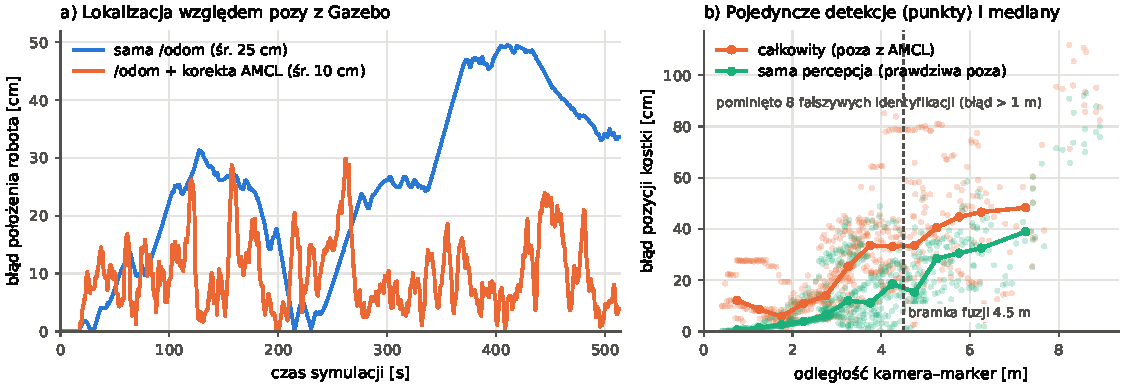
\includegraphics[width=\linewidth]{wykres_bledow.pdf}

\vspace{1mm}
\textbf{Rys. A1.} a) Błąd położenia robota względem pozy z Gazebo w przebiegu 514~s: sama odometria (śr. 25~cm, maks. 50~cm) i odometria z korektą map\ra{}odom z AMCL (śr. 10~cm, maks. 30~cm). b) Błąd pozycji kostki dla pojedynczych detekcji w funkcji odległości: całkowity (poza robota z AMCL) oraz samej percepcji (ta sama detekcja przeliczona z prawdziwą pozą robota). Linie to mediany w przedziałach 0.5~m. Błąd poprzeczny do promienia widzenia ma medianę 0.4~cm, więc prawie cały błąd leży w głębi. Pominięto 8 fałszywych identyfikacji ID~0 (błąd $>$1~m). Dane: \code{logi/pomiar/}, skrypt: \code{tools/plot_eval.py}.
\fi
\end{document}
